\chapter{Pattern comportamentali e costruzione di features}
\label{cap2}
Gli individui mostrano spesso pattern comportamentali nella scelta dei loro usernames. Questi pattern, risultanti in ridondanza di informazione, possono essere utili per identificare individui su diversi social networks.
I soggetti potrebbero evitare queste ridondanze selezionando username in modo che risultino completamente diversi dai loro altri usernames. In questa maniera gli username risulterebbero essere talmente differenti che, dato uno username, nessuna informazione riguardante gli altri usernames potrebbe essere estratta.
Idealmente per raggiungere questo stato di indipendenza tra usernames, l'individuo dovrebbe scegliere uno username che presenti entropia massima. Ovvero uno username composto da una lunga sequenza di caratteri, lunga quanto il massimo consentito dal sistema, senza ridondanze: una sequenza di caratteri completamente casuale.
Sfortunatamente, tutti questi requisiti non vengono incontro alle abilità umane. Gli esseri umani hanno difficoltà a memorizzare lunghe sequenze, con la possibilità della memoria a breve termine di ricordare 7$\pm$2 elementi\cite{miller1956magical}. Queste limitazioni risultano condurre gli individui a selezionare generalmente usernames \textit{non lunghi}, \textit{non casuali} e che presentano \textit{abbondante ridondanza}.
Queste proprietà possono essere catturate adottando features specifiche.

Possiamo suddividere questi pattern comportamentali in tre categorie:
\begin{enumerate}
  \item Pattern dovuti a limitazioni umane
  \item Fattori esogeni
  \item Fattori endogeni
\end{enumerate}

Discuteremo dei comportamenti di ognuna di queste categorie elencate e delle features che possono essere estrapolate sfruttando questi pattern.\newline Riportiamo anche qui alcune notazioni già accennate nel capitolo 1 per chiarezza. Useremo spesso in questo capitolo, e nei capitoli a venire, notazioni quali “individui” , “username candidate”, “prior username”.
Utilizzeremo la notazione \textit{SNS} intendendo \textit{Social Network Services}.
Ci riferiremo a un “individuo” \textit{i}, intendendo una persona umana, fisica, considerata nella sua singolarità. Utilizzeremo le parole “user” o “utente” per riferirci allo stesso concetto. Un individuo \textit{i}, potrebbe essere registrato a diversi SNS, per il quale tendenzialmente è richiesto selezionare uno username \textit{u}. Ci riferiremo all'insieme di tutti gli username conosciuti di \textit{i} con la notazione \textit{U\textsubscript{i}} “priors username” o semplicemente “priors”. Notare che \textit{U\textsubscript{i}} potrebbe essere un sottoinsieme di un insieme piú grande, con username addizionali, a noi però sconosciuti. Ci riferiremo invece a “username candidate” o semplicemente “candidate” o \textit{c\textsubscript{i}} intendendo uno username che si intende testare, ovvero capire se fa parte dell'insieme \textit{U\textsubscript{i}}.
Riassumendo, abbiamo:
\begin{itemize}
  \item \textit{I} si riferisce all'insieme di individui \textit{i}
  \item \textit{U\textsubscript{i}} riferisce all'insieme di username \textit{u} per \textit{i} o \textit{priors username}
  \item \textit{c\textsubscript{i}} si riferisce al \textit{candidate} per l'individuo \textit{i} con priors \textit{U\textsubscript{i}}
\end{itemize}


\section{Pattern dovuti a limitazioni umane}

In generale, come umani, noi abbiamo:

\begin{enumerate}
  \item Tempo e memoria limitati
  \item Conoscenza limitata
\end{enumerate}

Entrambe pregiudicano e influenzano i comportamenti nel selezionare i nostri username.
Presentiamo qui le features individuate per catturare questi pattern comportamentali.


\paragraph{Username identici (1 feature)}
Uno studio recente\cite{zafarani09} dimostra che il 59\% degli individui preferisce usare lo stesso username reiteratamente, principalmente per facilità nel ricordarlo. Quindi se un candidate username \textit{c\textsubscript{i}} compare tra i priors username \textit{U\textsubscript{i}}, vi è una forte indicazione che che potrebbe essere associato allo stesso individuo \textit{i} a cui sono associati i priors username. Considereremo dunque di utilizzare il numero di match esatti tra candidate username tra i prior usernames come feature.

\paragraph{Username Length Likelihood (6 feature)}
Allo stesso modo, gli utenti hanno tipicamente un insieme di potenziali usernames dal quale estraggono quando richiesto di crearne uno nuovo. Questi usernames hanno differenti lunghezze e dunque è possibile calcolarne una distribuzione. Consideriamo \textit{l\textsubscript{c}} la lunghezza del candidate username e \textit{l\textsubscript{u}} la lunghezza di uno username \textit{u} $\in$ \textit{U\textsubscript{i}}.
Assumiamo che per ogni nuovo username creato è probabile il verificarsi di\\
\centerline{$\min$\textit{l\textsubscript{u}} $\leq$ \textit{l\textsubscript{c}} $\leq$ $\max$\textit{l}\textsubscript{u}}
Ad esempio se un individuo è solito scegliere username di lunghezza 8 o 9 caratteri, è improbabile che questo consideri di crearne uno con lunghezze minori o maggiori.
Considereremo quindi le lunghezza del candidate username e la distribuzione delle lunghezze dei prior usernames come features. La distribuzione verrà rappresentata da un numero fisso di features, descrivendola come\\
\centerline{($\mathbb{E}$[\textit{l\textsubscript{u}}],$\sigma$[\textit{l\textsubscript{u}}], med[\textit{l\textsubscript{u}}],$\min$\textit{l\textsubscript{u}},$\max$\textit{l\textsubscript{u}})}

\paragraph{Unique username creation Likelihood (1 feature)}
Spesso gli utenti tendono a non creare nuovi username quando vogliono registrarsi a un SNS, ma preferiscono, se possibile, utilizzare uno username selezionato precedentemente. Siamo interessati a misurare lo sforzo che gli utenti sono disposti a mostrare nel creare nuovi username. Questo può essere approssimato dal numero di username unici (\textit{uniq(U)}) su la totalità dei priors username \textit{U}

\begin{gather*}
   \textit{uniqueness} = \frac{|\textit{uniq(U)}|}{|\textit{U}|}
\end{gather*}

\textit{Uniqueness} sarà una feature nel nostro insieme di feature. Si può pensare 1/\textit{uniqueness} come la media di volte in cui un individuo utilizza uno username su diversi SNS prima di decidere di crearne uno nuovo.

\section{Fattori esogeni}
I fattori esogeni sono comportamenti osservati dovuti a influenze culturali o in generale dall'ambiente in cui l'utente si trova e vive. Possiamo dividere i fattori esogeni in due categorie:

\begin{enumerate}
  \item Pattern di battitura
  \item Pattern linguistici
\end{enumerate}

\subsection{Pattern di battitura}
Si può pensare alla tastiera come un vincolo imposto dall'ambiente. È stato mostrato\cite{doctorow} l'impatto che la configurazione dei tasti di una tastiera ha sulla scelta di passwords e username, “grazie” a una massiva falla di sicurezza\footnote{http://leakedin.org}, che ha permesso di accedere a 6.5 milioni di passwords di altrettanti utenti di LinkedIn. Ad esempio \textbf{qwer1234} e \textbf{aoeusnth} sono due password molto conosciute per essere selezionate da utenti che utilizzano tastiere QWERTY e DVORAK rispettivamente. La maggior parte degli utenti utilizzano tastiere con disposizione dei tasti conosciute come QWERTY e DVORAK (o qualche variante come QWERTZ o AZERTY)\cite{keylayout}\newline
Le feature qui presentate, tentano di catturare questi schemi ricorrenti correlati alla tastiera. Si assume che le persone utilizzino entrambe le mani per digitare sulla tastiera e che siano a conoscenza della tecnica di dattilografia \textit{touch typing}\cite{touchtyping}. Elaboreremo queste feature per entrambe le configurazioni di tasti appena discusse.

\begin{figure}[bp!]
\centering
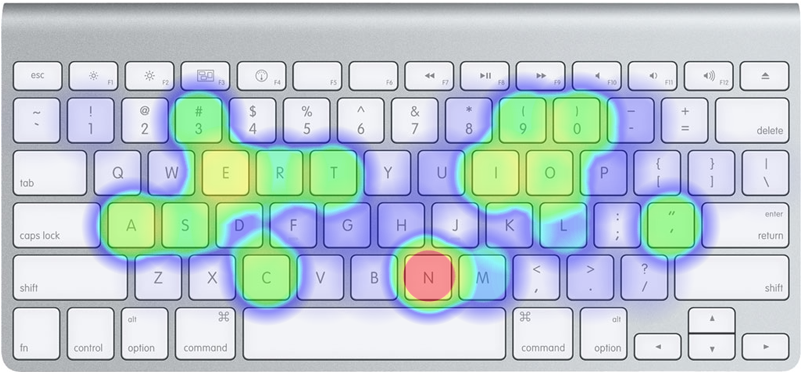
\includegraphics[width=90mm]{chapters/img/heatmapkey.png}
\caption{Una heatmap che rappresenta un esempio di pattern riscontrabile su tastiera  \label{overflow}}
\end{figure}

\paragraph{Stessa mano (12 feature)}
Siamo interessati a calcolare la percentuale di tasti digitati utilizzando la stessa mano usata per il tasto precedente, nel digitare uno username. Questo valore è inversamente proporzionale alla inclinazione dell'utente a cambiare mano nel digitare.

\paragraph{Stesse dita (12 feature)}
Siamo interessati a calcolare la percentuale di tasti digitati utilizzando lo stesso dito utilizzato per digitare il tasto precedente.

\paragraph{Ogni dito (96 feature)}
Con queste feature vogliamo calcolare la percentuale di tasti digitati per ogni dito. Ad esempio 15\% digitati con indice della mano sinistra, 2\% con il mignolo della mano destra, ecc... . I pollici non vengono conteggiati, in quanto dovrebbero venire utilizzati solamente per il tasto barra spaziatrice.

\paragraph{Spostamenti verticali (48 feature)}
Per queste features vogliamo calcolare la percentuale di tasti digitati su ogni fila orizzontale di tasti presente sulla tastiera, dove la riga superiore contiene i tasti numerici e le tre file sotto si dividono il resto dei caratteri. Con queste feature si intendono catturare i movimenti orizzontali delle dita sulla tastiera nel digitare gli username.

\paragraph{Distanza percorsa}
Questa feature rappresenta la distanza approssimata (in metri), percorsa per digitare uno username assumendo che un tasto di una tastiera standard misura 1.8cm$^2$, inclusi i margini attorno al tasto.\newline \newline
Per ogni campione, elaboreremo ognuna di queste feature per lo username candidate e ognuno dei priors username. Per ottenere un numero di feature eguale per ogni sample, in quanto ciascuno potrebbe avere un numero differente di priors, comprimeremo i valori calcolati per ogni prior username utilizzando la tecnica mostrata in 2.1, che ne calcola una distribuzione.

\subsection{Pattern linguistici}
Oltre a fattori ambientali, alcuni fattori culturali come il linguaggio, influenzano la scelta di uno username. Gli utenti utilizzano spesso la stessa lingua o lo stesso insieme di lingue nello scegliere uno username. Dunque, ci si aspetta un risultato piuttosto coerente se si osservano le lingue di piú username appartenenti allo stesso individuo. Per individuare la lingua di uno username potremmo utilizzare un sistema sviluppato da terzi. Solitamente si tratta di sistemi che inferiscono la lingua di un testo utilizzando classificatori addestrati su n-grammi estratti da corpus di varie lingue. A seconda della fase di apprendimento di questi classificatori, questi potranno essere capaci di riconoscere un insieme di lingue diverse, ma rimane impegnativo poterle riconoscere tutte. Un'altra sfida sottoposta a questi classificatori si propone quando vengono analizzate parole che potrebbero non seguire pattern statistici di alcun linguaggio, ad esempio sostantivi o luoghi. Per queste ragioni la feature non verrà implementata, ma verrà proposto un metodo che affronta questo problema da una diversa angolatura in seguito.


\section{Fattori endogeni}
I fattori endogeni giocano un ruolo molto importante nella selezione di uno username. Alcuni di questi fattori sono da attribuire a:

\begin{enumerate}
  \item Attributi personali (nome, età, sesso, ruolo, posizione lavorativa, ecc.)
  \item Casualità
  \item Usanze (abitudini, abbreviazioni, prefissi o suffissi etc.)
\end{enumerate}

\subsection{Attributi personali}
\paragraph{Informazioni personali (156 feature)}
Come menzionato, una delle problematicità di un modello per l'identificazione della lingua a partire da uno username si riscontra nell'individuare la lingua di nomi specifici, come luoghi o altri aspetti specifici dell'individuo che sta selezionando lo username. Ad esempio non sarebbe semplice inferire la lingua di uno username \textbf{R2D2}\footnote{R2-D2 è un personaggio robot nell'universo di StarWars} o \textbf{K2}\footnote{Montagna del Pakistan}. Ad ogni modo, i pattern presenti in queste parole possono essere catturati analizzando la distribuzione delle lettere dell'alfabeto. Ad esempio un utente che sceglie lo username \textbf{piccettino}\footnote{Piccettino è un personaggio appartenente all'universo di Rat-Man} il piú delle volte opterà per uno username con una distribuzione dell'alfabeto che presenta una probabilità doppia per le lettere ‘c’, ‘i’, ‘t’  rispetto alle altre lettere. Dunque, calcoliamo la distribuzione dell'alfabeto per ambedue i candidate username e prior username da utilizzare come feature. Questa metodologia viene usata come alternativa al sistema di riconoscimento delle lingue. Inoltre, il beneficio nell'utilizzare la distribuzione delle lettere dell'alfabeto non è solamente il fatto di essere lingua-indipendente, ma anche la capacità di carpire parole che hanno significato solo per l'utente.\newline
\subsection{Casualità}
\paragraph{Casualità degli username (6 feature)}
Come indicato precedentemente se un utente selezionasse uno username completamente casuale, non genererebbe alcuna ridondanza di informazione. Possiamo quantificare la casualità degli username di un individuo e considerarla come feature che misura il livello di privacy dell'individuo, che potrebbe aiutare nell'identificarlo. Per misurare la casualità, considereremo l'entropia\cite{thomcov} della distribuzione delle lettere dell'alfabeto che compongono lo username candidato come feature. Questa verrà calcolata anche per ogni prior username, risultando in una distribuzione di valori di entropia usando la tecnica di distribuzione sopra mostrata in 2.1.
\subsection{Usanze}
Alcuni utenti mostrano delle usanze o abitudini che, come la famosa espressione ricorda, sono dure a morire e vengono puntualmente ripresentate. Abitudini comuni comprendono:

\paragraph{Modifica username} Spesso gli utenti scelgono un nuovo username cambiando qualcosa del loro username precedente. Alcuni:\newline

\begin{enumerate}
    \item Aggiungono prefissi o suffissi, ad esempio \textbf{mattia} che diventa \textbf{mattia87}
  \item Abbreviano i loro username, ad esempio \textbf{mattia.dimauro} che diventa \textbf{mattiadmr}
  \item Alternano caratteri o inseriscono nuovi caratteri, come \textbf{mattia} che diventa \textbf{matt1a}
\end{enumerate}

Le feature elencate qui sotto cercano di carpire queste modifiche.

\paragraph{Prefissi e suffissi (5 feature)} Per individuare prefissi si può controllare se uno username è una sottostringa dell'altro. Dunque, si considera la lunghezza della massima sottostringa comune o LCS\footnote{Longest Common Substring} come feature informativa di simiglianza tra tra candidate e prior.

\paragraph{Abbreviazioni (5 feature)} Per individuare le abbreviazioni usiamo la lunghezza della massima sottosequenza\footnote{Longest Common Subsequence Utilizzato in bioinformatica per analizzare sequenze di DNA, e alla  base del tool \textit{diff} per comparare testi}, da non confondere con LCS, sensibile anche a lettere non consecutive che corrispondono in due stringhe. Questa viene calcolata per ogni prior username e ne viene elaborata la distribuzione.

\paragraph{Caratteri invertiti o nuovi inserimenti (10 feature)} Per individuare i caratteri invertiti o aggiunti faremo uso di alcune metriche di similarità su stringhe. Queste sono tecniche per quantificare la dissimilarità tra due stringhe. In particolare utilizzeremo la distanza di Levensthein, una metrica per misurare la differenza tra due sequenze, e l’indice di Jaccard, un indice statistico utilizzato per comparare la similarità e la diversità di insiemi campionari. L'indice di Jaccard per misurare la similarità degli username non viene utilizzato come feature nel lavoro di Zafarani, a noi sembrava opportuno utilizzarla in quanto identificativa sul problema di classificazione affrontato, come vedremo meglio nel capitolo seguente.
